%
% loesung.tex -- Beispiel-File für die Beschreibung der Loesung
%
% (c) 2020 Prof Dr Andreas Müller, Hochschule Rapperswil
%
\section{Lösung
\label{quadratur:section:loesung}}
\rhead{Lösung}
\subsection{Anwendung der Gauss-Legendre-Formel
\label{quadratur:subsection:gausslegendreanwendung}}
In diesem Unterabschnitt versuchen wir, die Verwendung der Gauss-Legendre-Formel in einem
einfachen Beispiel herzuleiten, hierzu wird wieder die Funktion  
$f(x) = \sqrt{(1-x^2)}$ verwendet und 
wir berechnen das Integral mit vier Stützstellen.
In der Tabelle~\ref{buch:table:gaussbeispielwerte} sind die Werte der 
Stützstellen und der Gewichte für dieses Beispiel angegeben.
Die Berechnung der Stützstellen, der Gewichte
und die verschiedenen Formen der Gauss-Quadratur werden in den folgenden Abschnitten 
hergeleitet.
\begin{table}
    \centering
    \begin{tabular}{|c|c|}
        \hline
        Stützstellen $x_{i}$ & Gewichte $A_{i}$ \\
        \hline
        $-0.861136 $ & $ 0.347855 $ \\
        $-0.339981 $ & $ 0.652145 $ \\
        $\phantom{-} 0.339981 $ & $ 0.652145 $ \\
        $\phantom{-} 0.861136 $ & $ 0.347855 $ \\
        \hline
    \end{tabular}
    \caption{Werte für vier Stützstellen und deren Gewichte
    \label{buch:table:gaussbeispielwerte}}    
\end{table}
In der Abbildung~\ref{quadratur:figure:gausslegendre1} sind die vier Stützstellen 
ersichtlich.
\begin{figure}
    \centering
    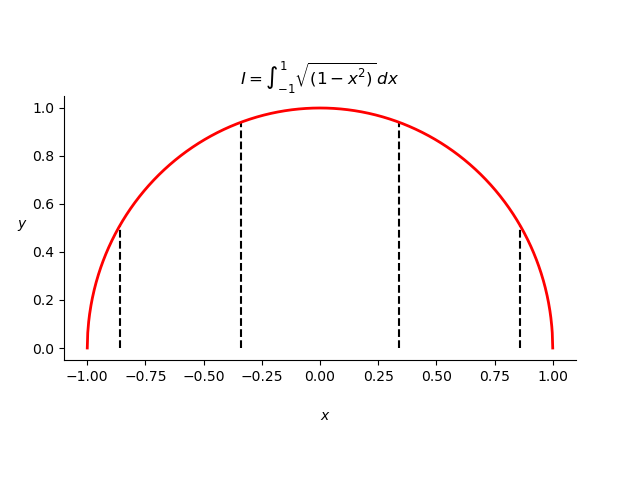
\includegraphics[scale=0.7]{papers/quadratur/figures/GaussLegendre1.png}
    \caption{ Position der Stützstellen
    \label{quadratur:figure:gausslegendre1}}
\end{figure}
Die Fläche unter dem Graphen lässt sich nun mit der Formel 
\begin{equation}
    I 
    =
    \int_{-1}^{1} f(x) 
    \approx
    \sum_{i=0}^{n} A_{i} f(x_{i})
\end{equation}
berechnen, indem man die Stützstellen $x_{i}$ und die Gewichte $A_{i}$ einsetzt.
Man erhält
\begin{align}
    \centering
    I 
    &\approx 
    0.347855 \cdot \sqrt{1-(-0.861136)^{2}} 
    \notag
    \\
    &+ 
    0.652145 \cdot \sqrt{1-(-0.339981)^{2}} 
    \notag
    \\
    &+ 
    0.652145 \cdot \sqrt{1-(0.339981)^{2}} 
    \notag
    \\
    &+ 
    0.347855 \cdot \sqrt{1-(0.861136)^{2}} 
    \notag
    \\
    &\approx 2 \cdot 0.652145 \cdot \sqrt{1-(0.339981)^{2}} + 2 \cdot 0.347855 \cdot \sqrt{1-(0.861136)^{2}} 
    \notag
    \\
    &\approx 1.226596 + 0.386863 
    \notag
    \\
    &\approx 1.580278.
\end{align}
Das Resultat $1.580278$ ist eine genauere Annäherung an die 
tatsächliche Fläche $1.570796$ als die Resultate der Trapezformel. 

\subsection{Berechnung der Position der Stützstellen
\label{quadratur:subsection:stützstellenberechnung}}
Um die Position der Stützstellen zu bestimmen, benötigt man zuerst die Anzahl Stützstellen, 
die für die Quadratur einer Funktion benötig werden.
Wie im Abschnitt~\ref{quadratur:section:problemstellung} erwähnt, 
kann man mit $n$ Stützstellen das Integral eines Polynoms vom Grad $2n-1$ exakt berechnen.
Anders ausgedrückt: Hat man ein Polynom vom Grad $g$, 
benötigt man für eine exakte Berechnung des Integrals $\frac{g+1}{2}$ Stützstellen.
Hat man eine Funktion, die sich nicht als Polynom darstellen lässt, 
kann man die Funktion durch ein Polynom annähern, 
oder die Anzahl benötigter Stützstellen schätzen.
Falls man die Anzahl Stützstellen schätzt, ist darauf zu achten, 
dass eine grössere Anzahl zwar die Genauigkeit der Quadratur erhöht,
aber auch der Berechnungsaufwand grösser wird.

\subsubsection{Beispiel: Polynom vom Grad $7$}
Angenommen, man hat die Funktion $f(x) = 5 \cdot x^{7} + 2 \cdot x^{5} - 8 \cdot x^{3} + x + 3$.
Der Grad der Funktion lässt sich aus dem höchsten vorkommenden Exponenten von $x$ ableiten,
also $7$.
Für ein Polynom vom Grad $7$ werden $\frac{7+1}{2} = 4$ Stützstellen benötigt.
In der Abbildung~\ref{quadratur:figure:polynom} ist die Funktion mit den vier 
Stützstellen ersichtlich.
\begin{figure}
    \centering
    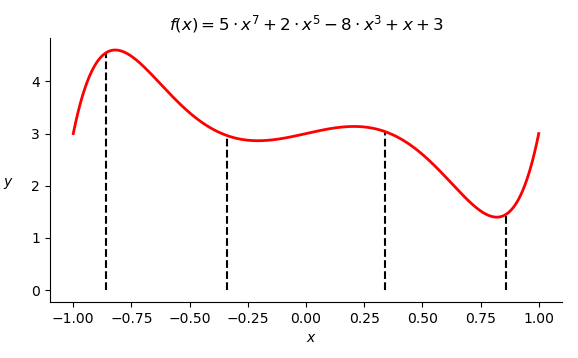
\includegraphics[scale=0.7]{papers/quadratur/figures/polynom.png}
    \caption{ Funktion des Polynom mit vier Stützstellen
    \label{quadratur:figure:polynom}}
\end{figure}

\subsubsection{Annäherung von Funktionen durch Polynome}
Im Kapitel~\ref{chapter:interpolation} wurde bereits gezeigt, 
wie man eine Funktion $f(x)$ durch ein Polynom 
\begin{equation}
    p(x) = a_{0} + a_{1}x + a_{2}x^{2} + ... + a_{n}x^{n}
\end{equation}
annähern kann. Möchte man nun das Integral $\int_{-1}^{1} f(x) \, dx$ annähern, 
muss man dazu die Integrale 
\begin{equation}
    \int_{-1}^{1} p(x)\,dx 
    =
    a_{0} \int_{-1}^{1} 1\,dx
    +
    a_{1}\int_{-1}^{1} x\,dx 
    + 
    a_{2}\int_{-1}^{1} x^{2} \,dx  
    +
    ... 
    +
    a_{n}\int_{-1}^{1} x^{n}\,dx 
\end{equation}
berechnen können. Diese Berechnungen kann man durch die allgemeine Formel
\begin{equation}
    \int_{-1}^{1} x^{k}\,dx 
    = 
    \bigg[\frac{1}{k+1} x^{k+1}\bigg]_{-1}^{1}
    =
    \frac{1^{k+1} - (-1)^{k+1}}{k+1}  
\end{equation}
dargestellt werden.

Man kann hier erkennen, dass:
\begin{equation}
    \int_{-1}^{1} x^{k}\,dx 
    =
    \begin{cases}
        0&\qquad k \; \text{ungerade}\\
        \frac{2}{k+1}&\qquad k \; \text{gerade}
        \end{cases}  
\end{equation}
Die Erkennntniss, dass ungerade Terme in der Berechnung 
des Integrals eines Polynoms verschwinden, 
erklärt, warum für die Quadratur eines Polynoms nur $\frac{n+1}{2}$ 
Stützstellen benötigt werden. Es müssen nur die geraden Terme evaluiert werden,
da:
\begin{equation}
    \int_{-1}^{1} p(x)\,dx 
    =
    a_{0} \int_{-1}^{1} 1\,dx
    +
    0
    + 
    a_{2}\int_{-1}^{1} x^{2} \,dx  
    +
    0
    +
    ... 
    +
    a_{n}\int_{-1}^{1} x^{n}\,dx
\end{equation}
Weiss man, wieviele Stützstellen $n$ man für die Berechnung der Quadratur verwenden möchte,
kann man die Position der Stützstellen berechnen. 
Dafür hat man drei Möglichkeiten, welche nachfolgend erklärt werden.

\subsubsection{Substitution der Polynome}
Eine Möglichkeit für die Berechnung der Stützstellen (und Gewichte) ist, in der Formel
\begin{equation} \label{quadratur:equation:polynomsubstitution}
    \int_{a}^{b}w(x)P_{m}(x)\, dx = \sum_{i=0}^{n}A_{i}P_{m}(x_{i}), \; m \leq 2n + 1
\end{equation}
die Polynome $P_{m}$ durch
\begin{equation}
     P_{0}(x) = 1, P_{1}(x) = x, \dots , P_{2n+1}(x) = x^{2n+1}
\end{equation}
zu ersetzen und die resultierenden $2n+2$ Gleichungen 
\begin{equation}
    \int_{a}^{b}w(x)x^{j}\,dx = \sum_{i=0}^{n} A_{i}x_{i}^{j}, j = 0, 1, \dots , 2 n + 1
\end{equation}
für die Unbekannten $x_{i}$ und $A_{i}$ zu lösen.

Nimmt man beispielsweise an, dass $w(x) = x, a = -1, b = 1$ und $n = 1$, 
dann ist das resultierende Gleichungssystem:
\begin{align}
    \int_{-1}^{1} x \phantom{x^{0}} \, dx &= A_{0}\phantom{x^{0}} + A_{1}\phantom{x^{0}} \\
    \int_{-1}^{1} x x \, dx &= A_{0}x_{0} + A_{1}x_{1} \\
    \int_{-1}^{1} x x^{2} \, dx &= A_{0}x_{0}^{2} + A_{1}x_{1}^{2} \\
    \int_{-1}^{1} x x^{3} \, dx &= A_{0}x_{0}^{3} + A_{1}x_{1}^{3} 
\end{align}
Löst man die Integrale, erhält man
\begin{align}
    A_{0}\phantom{x^{0}} + A_{1}\phantom{x^{0}} &= 0 \\
    A_{0}x_{0} + A_{1}x_{1} &= \frac{2}{3} \approx 0.66667 \\
    A_{0}x_{0}^{2} + A_{1}x_{1}^{2} &= 0 \\
    A_{0}x_{0}^{3} + A_{1}x_{1}^{3} &= \frac{2}{5} = 0.4
\end{align}
daraus ergibt sich die Lösung
\begin{align}
    A_{0} &= \phantom{-}\frac{\sqrt{\frac{5}{3}}}{3} & x_{0} &= -\sqrt{\frac{3}{5}} & \\
    A_{1} &= -\frac{\sqrt{\frac{5}{3}}}{3} & x_{1} &= \phantom{-}\sqrt{\frac{3}{5}} &
\end{align}
Setzt man diese werte in die Integrationsformel ein, so wird die Formel
\begin{equation}
    \int_{-1}^{1}x \cdot f(x)\,dx \approx \frac{1}{3} \bigg[ (\sqrt{\frac{5}{3}})f(-\sqrt{\frac{3}{5}}) + (-\sqrt{\frac{5}{3}})f(\sqrt{\frac{3}{5}})\bigg]
\end{equation}
Man kann sehen, dass diese Methode für die Berechnung der Stützstellen 
für grosse $n$ sehr schnell viel Zeit beansprucht.
Die anderen Methoden für die Bestimmung der Stützstellen 
und Gewichte sind effektiver und in der Anwendung einfacher.

\subsubsection{Werte in der Tabelle nachschlagen}
Für die gängigsten Formen der Gauss-Quadratur existieren Tabellen mit vorberechneten Werten für die
Position der Stützstellen und deren Gewichte. 
Die Tabellen sind sehr präzise und für die ersten hundert $n$ vorgerechnet.
Ausserdem gibt es Programme, welche für beliebige $n$ die dazugehörigen 
Stützstellen und Gewichte berechnen. 
In der Tabelle~\ref{buch:table:gaussabscissenwerte} sind die Werte für $n \leq 5$ beschrieben.
\begin{table}
    \centering
    \begin{tabular}{|c|c|}
        \hline
        $n$ & Stützstellen $x_{i}$ für $n$ \\
        \hline
        $0$ & $ \phantom{-} 0.00000 $ \\
        \hline
        $1$ & $ \pm 0.57735 $ \\
        \hline
        $2$ & $ \pm 0.77460 $ \\
            & $ \phantom{-} 0.00000 $ \\
        \hline
        $3$ & $ \pm 0.86114 $ \\
            & $ \pm 0.33998 $ \\
        \hline
        $4$ & $ \pm 0.90618 $ \\
            & $ \pm 0.53847 $ \\
            & $ \phantom{-} 0.00000 $ \\
        \hline
        $5$ & $ \pm 0.93247 $ \\
            & $ \pm 0.66121 $ \\
            & $ \pm 0.23862 $ \\
        \hline
    \end{tabular}
    \caption{Werte für Stützstellen $x_{i}$ der Gaussquadratur für $n \leq 6$
    \label{buch:table:gaussabscissenwerte}}    
\end{table}

\subsubsection{Berechnen durch Formel}
Die Position der Stützstellen lässt sich mit der Formel
\begin{equation*}
    \int_{-1}^{1} P(x) \cdot x^{j} \, dx = 0
\end{equation*}
mit
\begin{equation*}
    j = 0, 1, 2, ... n - 1
\end{equation*}
und 
\begin{equation}
    P(x) = (x - x_{1})(x - x_{2}) ... (x - x_{n})
\end{equation}
berechnen. Um die Formel zu verstehen, werden einige Grundkenntnisse für 
orthogonale Polynome und deren Beziehung zur Gauss-Quadratur vorausgesetzt.
Da aber für die häufigsten Formen der Gauss-Quadratur 
(Siehe Abschnitt ~\ref{quadratur:subsection:gaussformen}) bereits vorberechnete
Tabellen für die Stützstellen und Gewichte existieren muss man die Theorie
für die Anwendung der Formeln nicht verstehen. Für interessierte Leser sind 
die wichtigsten Eigenschaften von orthogonalen Polynomen im nächsten 
Abschnitt genäuer erläutert.

\subsubsection{Beispiel: Berechnung für zwei Stützstellen}
Möchte man die Position für zwei Stützstellen berechnen, sieht die Formel folgendermassen aus:
\begin{equation}
    P(x) = (x - x_{1})(x - x_{2})
\end{equation}
und man erhält für $j = 0,1$ die beiden Gleichungen
\begin{align}
    j &= 0: & \int_{-1}^{1}P(x)\phantom{x^{1}}\,dx  &= \int_{-1}^{1}(x - x_{1})(x - x_{2})\phantom{x} \; dx = 0 & \\
    j &= 1: & \int_{-1}^{1}P(x)x^{1}\,dx            &= \int_{-1}^{1}(x - x_{1})(x - x_{2})x \; dx = 0 &
\end{align}
Löst man das Integral, erhält man:
\begin{align}
    j  &= 0: & \frac{1}{3} + x_{1}x_{2} &= 0 & \\
    j  &= 1: & \frac{2}{3}(x_{1}+x_{2}) &= 0 &
\end{align}
Umgeformt erhält man:
\begin{equation}
    x_{1}x_{2} = -\frac{1}{3}
    \;
    \text{und}
    \;
    x_{1}+x_{2} = 0
\end{equation}
Somit sind $ x_{1} $ und $ x_{2} $:
\begin{equation*}
    x_{1} = -\frac{1}{\sqrt{3}} \approx -0.55735
\end{equation*}
\begin{equation}
    x_{2} = \phantom{-} \frac{1}{\sqrt{3}} \approx \phantom{-}0.55735
\end{equation}

\subsection{Orthogonale Polynome
\label{quadratur:subsection:orthogonalepolynome}}

\subsubsection{Grundlagen orthogonale Polynome}
Orthogonale Polynome werden in der mathematischen und 
numerischen Analysis oft verwendet.
In der numerischen Integration entsprechen die Nullstellen
der Orthogonalen Polynome den Stützstellen der Gaussquadratur.
Zwei Polynome $\phi_{m}(x)$ und $\phi_{n}(x)$ 
($n$ und $m$ ist hierbei der Grad des Polynoms) formen ein 
orthogonales Paar im Intervall $(a, b)$ im Bezug auf die Gewichtungsfunktion
$w(x)$ falls:
\begin{equation}
    \int_{a}^{b} w(x) \phi_{m}(x) \phi_{n}(x)\,dx = 0 \, , m \neq n
\end{equation}
Orthogonalpolynome sind abgesehen von einem konstanten Faktor, 
der über die Normierung der Polynome ermittelt wird,
über die Wahl der Gewichtungsfunktion und der Grenzen des Integrals $a, b$, festgelegt.
Klassische Orthogonalpolynome sind nach bekannten Mathematikern 
benannt und in der Tabelle~\ref{buch:table:orthogonalpolynomials} mit ihren
Eigenschaften beschrieben.
\begin{table}
    \centering
    \begin{tabular}{|l|>{$}c<{$}|>{$}c<{$}|>{$}c<{$}|>{$}c<{$}|}
        \hline
        Name & \text{Symbol} & a & b & w(x) \\
        \hline
        Legendre & p_{n(x)} & -1 & 1 & 1 \\
        Chebyshev & T_{n}(x) & -1 & 1 & (1-x^{2})^-1/2 \\
        Laguerre & L_{n}(x) & \phantom{-}0 & \infty & e^{-x} \\
        Hermite & H_{n}(x) & -\infty & \infty & e^{-x^{2}} \\
        \hline
    \end{tabular}
    \caption{Klassische Orthogonalpolynome
    \label{buch:table:orthogonalpolynomials}}    
\end{table}
Weiterhin haben orthogonale Polynome rekursive Beziehungen zueinander, das heisst,
dass mit der Formel
\begin{equation}
    a_{n}\phi_{n+1}(x) = (b_{n} + c_{n}x)\phi_{n}(x) - d_{n}\phi_{n-1}(x)
\end{equation}
mit den ersten beiden Orthogonalpolynomen weitere Polynome berechnet werden können. 
Die Koeffizienten für die Rekursionsformel finden sich in der 
Tabelle~\ref{buch:table:orthogonalcoefficients}
\begin{table}
    \centering
    \begin{tabular}{|l|>{$}c<{$}|>{$}c<{$}|>{$}c<{$}|>{$}c<{$}|>{$}c<{$}|>{$}c<{$}|}
        \hline
        Name & \phi_{0}(x) & \phi_{1}(x) & a_{n} & b_{n} & c_{n} & d_{n} \\
        \hline
        Legendre & 1 & x & n + 1 & 0 & 2n + 1 & n \\
        Chebyshev & 1 & x & 1 & 0 & 2 & 1 \\
        Laguerre & 1 & 1 - x & n + 1 & 2n + 1 & -1 & n \\
        Hermite & 1 & 2x & 1 & 0 & 2 & 2 \\
        \hline
    \end{tabular}
    \caption{Koeffizienten für die berechnung von Orthogonalpolynomen
    \label{buch:table:orthogonalcoefficients}}    
\end{table}

\subsubsection{Für die Gaussquadratur relevante Eigenschaften}

Ein orthogonales Polynom $\phi_{n}(x)$ vom Grad $n$ hat $n$ reelle, 
unterschiedliche Nullstellen im Intervall $(a, b)$.
Diese Eigenschaft ist für die Gaussquadratur relevant, 
da für eine Gauss-Quadraturformel vom Grad $n$ für die exakte Berechnung 
des Integrals diejenigen Abszissenwerte $x_{i}$ benötigt werden, 
welche den Nullstellen des $n-$ten orthogonalen Polynoms $P_{n}$ entsprechen.
Weiterhin liegen die Nullstellen Polynoms $\phi_{n}(x)$ zwischen den Nullstellen des Polynoms $\phi_{n+1}(x)$.
Diese Eigenschaft erlaubt es, den Grad $n$ des Polynoms zu erhöhen und man erhält dadurch 
mehr Nullstellen, welche den Stützstellen $x_{i}$ der Gauss-Quadraturformel entsprechen.

Ein beliebiges Polynom $P_{n}(x)$ kann in der Form 
$P_{n}(x) = \sum_{i=0}^{n} c_{i}\phi_{i}(x)$ ausgedrückt werden.
Anders ausgedrückt, lässt sich durch diese Eigenschaft ein beliebiges Polynom als
Linearkombination von Orthogonalpolynomen darstellen. 
Somit lässt sich das Integral für beliebige Polynome mit der Gaussquadratur exakt berechnen.

In der Abbildung~\ref{quadratur:figure:legendrepolynomial} sind die ersten vier
Legendre-Polynome abbgebildet. Man kann darin sehr gut sehen, 
dass die Positionen der Nullstellen den in der 
Tabelle~\ref{buch:table:gaussabscissenwerte} genannten Stützstellen $x_{i}$ 
entsprechen und dass die Nullstellen eines Polynoms $P_{n}$ zwischen denen 
eines Polynoms $P_{n+1}$ liegen.

\begin{figure}
    \centering
    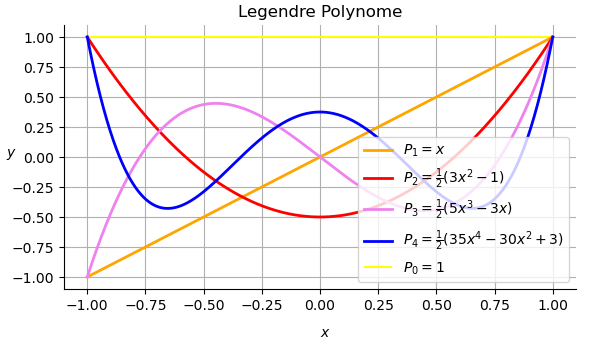
\includegraphics[scale=0.7]{papers/quadratur/figures/Legendrepolynomial.png}
    \caption{ Die Ersten vier Legendre-Polynome
    \label{quadratur:figure:legendrepolynomial}}
\end{figure}

\subsection{Berechnung der Gewichte an den Stützstellen
\label{quadratur:subsection:gewichtsberechnung}}
Auch für die Bestimmung der Gewichte an den berechneten Stützstellen kann man entweder
in einer vorberechneten Tabelle die Werte nachschlagen, oder die Gewichte selber berechnen.

\subsubsection{Tabelle für die Gewichte}
In der Tabelle~\ref{buch:table:gaussgewichtwerte} sind für $ n \leq 5 $ die Gewichte $A_{i}$
an den Stützstellen $x_{i} $ angegeben.

\begin{table}
    \centering
    \begin{tabular}{|c|c|c|}
        \hline
        $n$ & Stützstellen $x_{i}$ für $n$ & Gewichte $A_{i}$\\
        \hline
        $0$ & $ \phantom{-} 0.00000 $ & $ 2.00000 $ \\
        \hline
        $1$ & $ \pm 0.57735 $ & $ 1.00000 $ \\
        \hline
        $2$ & $ \pm 0.77460 $ & $ 0.55556 $ \\
            & $ \phantom{-} 0.00000 $ & $ 0.88889 $ \\
        \hline
        $3$ & $ \pm 0.86114 $ & $ 0.34785 $ \\
            & $ \pm 0.33998 $ & $ 0.65215 $ \\
        \hline
        $4$ & $ \pm 0.90618 $ & $ 0.23693 $ \\
            & $ \pm 0.53847 $ & $ 0.47863 $ \\
            & $ \phantom{-} 0.00000 $ & $ 0.56889 $ \\
        \hline
        $5$ & $ \pm 0.93247 $ & $ 0.17132 $ \\
            & $ \pm 0.66121 $ & $ 0.36076 $ \\
            & $ \pm 0.23862 $ & $ 0.46791 $ \\
        \hline
    \end{tabular}
    \caption{Werte für Stützstellen $x_{i}$ und Gewichte $A_{i}$ der Gaussquadratur für $n \leq 6$
    \label{buch:table:gaussgewichtwerte}}    
\end{table}

\subsubsection{Berechnen der Gewichte}
Die Gewichte an den Stützstellen lässt sich mit der Formel
\begin{equation*}
    A_{j} = \int_{-1}^{1} l_j(x) \, dx
\end{equation*}
mit
\begin{equation*}
    j = 1, 2, ... , n
\end{equation*}
und 
\begin{equation}
    l_{j}(x) := \prod_{0 \leq m \leq k, \, m \neq j} \frac{x - x_{m}}{x_{j} - x_{m}}
\end{equation}
berechnen.

Die Formel lässt sich mit der im Kapitel~\ref{chapter:interpolation} genannten 
Interpolationspolynom herleiten.
Für die Funktion $f(x)$ mit Stützstellen $x_{i}$ ist das Interpolationspolynom
\begin{equation}
    p(x) = \sum_{i=0}^{n} f(x_{i})l_{i}(x)
\end{equation}
und das Integral ist 
\begin{align}
    \int_{-1}^{1}f(x)\,dx &\approx \int_{-1}^{1}p(x)\,dx \\
    &= \int_{-1}^{1} \sum_{i=0}^{n} f(x_{i}) l_{i}(x) \,dx \\
    &= \sum_{i=0}^{n} f(x_{i}) \cdot \int_{-1}^{1}  l_{i}(x) \,dx
\end{align}
wobei $\int_{-1}^{1}  l_{i}(x) \,dx = A_{i}$.

\subsubsection{Beispiel: Berechnung der Gewichte für zwei Stützstellen}
In der Beispielberechnung der Stützstellen im
Abschnitt~\ref{quadratur:subsection:stützstellenberechnung} sieht man, dass sich die 
Stützstellen an den Punkten $x_{1} = -\frac{1}{\sqrt{3}} $ und $x_{2} = \frac{1}{\sqrt{3}} $ befinden.

Die Formeln für die Berechnung der Gewichte $A_{1}$ und $A_{2}$ sind:
\begin{equation*}
    A_{1} = \int_{-1}^{1} \frac{x - x_{2}}{x_{1} - x_{2}} \, dx
\end{equation*}
und
\begin{equation}
    A_{2} = \int_{-1}^{1} \frac{x - x_{1}}{x_{2} - x_{1}} \, dx
\end{equation}
setzt man die Werte für $x_{1}$ und $x_{2}$ in die Formeln ein, erhält man:
\begin{equation*}
    A_{1} = \int_{-1}^{1} \frac{x - \frac{1}{\sqrt{3}}}{\frac{-1}{\sqrt{3}} - \frac{1}{\sqrt{3}}} \, dx
\end{equation*}
\begin{equation}
    A_{2} = \int_{-1}^{1} \frac{x - \frac{-1}{\sqrt{3}}}{\frac{1}{\sqrt{3}} - \frac{-1}{\sqrt{3}}} \, dx
\end{equation}
vereinfacht man die Terme, erhält man:
\begin{equation*}
    A_{1} 
    =
    \int_{-1}^{1} -\frac{1}{2} 
    \cdot \sqrt{3} 
    \cdot \bigg(x - \frac{1}{\sqrt{3}}\bigg)
    \, dx
    =
    -\frac{\sqrt{3}}{2} 
    \bigg(
    \cdot \int_{-1}^{1}x\,dx
    -
    \frac{1}{\sqrt{3}} 
    \cdot \int_{-1}^{1}1\,dx
    \bigg)
\end{equation*}
\begin{equation}
    A_{2} 
    =
    \int_{-1}^{1} \frac{1}{2} 
    \cdot \sqrt{3}  
    \cdot \bigg(x + \frac{1}{\sqrt{3}}\bigg)
    \, dx
    =
    \frac{\sqrt{3}}{2} 
    \bigg(
    \cdot \int_{-1}^{1}x\,dx
    +
    \frac{1}{\sqrt{3}} 
    \cdot \int_{-1}^{1}1\,dx
    \bigg)
\end{equation}
$\int_{-1}^{1}x\,dx$ ist $0$ und $\int_{-1}^{1}1\,dx$ ist $2$, somit:
\begin{equation*}
    A_{1} 
    =
    -\frac{\sqrt{3}}{2} 
    \cdot 
    \bigg( 0
    -
    \frac{1}{\sqrt{3}} 
    \cdot 2
    \bigg)
    =
    1
\end{equation*}
\begin{equation}
    A_{2} 
    =
    \frac{\sqrt{3}}{2} 
    \cdot
    \bigg( 0
    +
    \frac{1}{\sqrt{3}} 
    \cdot 2
    \bigg)
    = 
    1
\end{equation}
es folgt somit, dass
\begin{equation}
    I 
    \approx 
    f(x_{1})+f(x_{2}) 
    = 
    f(-\frac{1}{\sqrt{3}})
    +
    f(\frac{1}{\sqrt{3}})
\end{equation}


\subsection{Formen der Gauss-Quadratur
\label{quadratur:subsection:gaussformen}}
Wie im Abschnitt~\ref{quadratur:subsection:stützstellenberechnung}, 
Orthogonale Polynome, bereits angedeutet, 
gibt es verschiedene Ausprägungen der Gauss-Integration.
Für verschiedene Folgen von Orthogonalpolynomen gibt es eine dazugehörige
Form der Gaussquadratur mit eigenen Grenzwerten und Berechnungsformeln.
Die vier häufigsten Formen sind in der Tabelle~\ref{buch:table:gaussformen} abgebildet.
\begin{table}
    \begin{tabular}{|l|>{$}c<{$}|>{$}c<{$}|>{$}l<{$}|}
        \hline
        \text{Name} &  \text{Untere Grenze} & \text{Obere Grenze} & \text{Formel} \\
        \hline  
        \text{Legendre} & -1 & 1 & p_{n}(x) = \int_{-1}^{1} f(x)\,dx \approx \sum_{i=0}^{n} A_{i} f(x_{i}) \\
        \text{Chebyshev} &  -1 & 1 & T_{n}(x) = \int_{-1}^{1} (1-x^{2})^{-1/2} f(x)\,dy \approx \frac{\pi}{n+1} \sum_{i=0}^{n} f(x_{i}) \\
        \text{Laguerre} &  0 & \infty & L_{n}(x) = \int_{0}^{\infty} e^{-x} f(x)\,dx \approx \sum_{i=0}^{n} A_{i} f(x_{i}) \\
        \text{Hermite} & -\infty & \infty & H_{n}(x) = \int_{-\infty}^{\infty} f(x)\,dx \approx \sum_{i=0}^{n} A_{i} f(x_{i})\\
        \hline
    \end{tabular}
    \caption{Formen der Gauss-Quadratur
    \label{buch:table:gaussformen}}   
\end{table}
In den bisherigen Beispielen wurde die Gaussformel mit der Legendre Form, auch Gauss-Legendre-Formel genannt, verwendet.
Interessant ist bei der Gauss-Chebyshev Formel, 
dass für die Berechnung des Integrals keine Gewichte berechnet werden müssen,
sondern dass für jedes $x_{i}$ das selbe Gewicht $\frac{\pi}{n+1}$ verwendet werden kann.
Ausserdem lassen sich die Stützstellen $x_{i}$ mit der Formel
\begin{equation}
    x_{i} = \cos \frac{(2i+1)\pi}{2n+2}
\end{equation}
berechnen und sind symetrisch um $x = 0$ verteilt.
Die Gauss-Laguerre Formel verwendet für die Bestimmung der Stützstellen die Laguerre-Polynome.
Diese Stützstellen liegen alle auf dem Intervall $[0, \infty]$

Möchte man nun ein beliebiges Integral mittels der Gaussquadratur berechnen,
deren Grenzwerte nicht zu den in der Tabelle~\ref{buch:table:gaussformen} 
dargestellten Formeln passt, 
abgesehen von weiteren hier nicht genannten Formen, 
muss man die Grenzwerte $(a, b)$ gemäss dem Folgenden Beispiel
auf den Bereich $(-1, 1)$ abbilden.

\subsubsection{Vorgehen bei Integralgrenzen, die nicht durch die Tabelle abgedeckt werden}

Angenommen man hat ein Integral
\begin{equation}
    \int_{a}^{b}f(\xi)\,d\xi
\end{equation}
Mit der Transformation
\begin{equation}
    \xi = \frac{b + a}{2} + \frac{b - a}{2} x    
\end{equation}
wird $d\xi = dx(b - a)/2$, und die Quadraturformel wird
\begin{equation}
    \int_{a}^{b}f(\xi)\,d\xi 
    =
    \frac{b - a}{2} \int_{-1}^{1}f\bigg(\frac{b - a}{2}x + \frac{b + a}{2}\bigg)\, dx 
    \approx
     \frac{b - a}{2} \sum_{i=1}^{n} A_{i}f\bigg(\frac{b - a}{2}x_{i} + \frac{b + a}{2}\bigg)
\end{equation}

\subsection{Fehler der Gauss-Quadratur
\label{quadratur:subsection:gaussfehler}}
Wie im Abschnitt~\ref{quadratur:subsection:stützstellenberechnung} erklärt,
lassen sich Polynome mit der Gauss-Quadratur exakt berechnen. 
Der Fehler für die Annäherung eines Integrals mittels eines Polynoms liegt
also in der Wahl des Annäherungspolynoms und ein Fehler in der Berechnung des Integrals.
Diesen Fehler können wir mit den im Abschnitt~\ref{buch:section:interpolation:fehler}
hergeleiteten Methoden ermitteln.
Weiterhin gibt es in der Gaussquadratur eigene Methoden, 
um den Fehler der Quadratur zu ermitteln. 
Die einfachere Methode ist, für eine Quadratur mit $n$ Stützstellen eine weitere
Quadratur mit $n+1$ Stützstellen durchzuführen und von der ersten Quadratur zu
subtrahieren. Die komplexere Methode ist, 
die Fehlerformel für die Gauss-Quadraturformel anzuwenden. 

\subsubsection{Fehlerrechnung mittels Quadratur höherer Ordung}

In der Praxis ist diese Methode für die Berechnung des Fehlers der Gaussquadratur
simpler und schneller in der Anwendung, da die Fehlerformel der Gaussquadratur
von der jeweiligen Methode der Gaussquadratur (Legendre, Laguerre, etc.) abhängt.
Für eine Gauss-Legendre-Quadratur 
\begin{equation}
    I 
    = 
    \int_{-1}^{1}f(x)\,dx 
    \approx 
    \sum_{i=1}^{n}A_{i}f(x_{i})
\end{equation}
kann der Fehler mit der Formel
\begin{equation}
    E 
    \approx 
    \sum_{i=1}^{n}A_{i}f(x_{i})
    -
    \sum_{i=1}^{n+1}A_{i}f(x_{i})
\end{equation}
approximiert werden. Für $n = 4$ wird die Fehlerrechnung 
\begin{gather*}
    E
    \approx
    \sum_{i=1}^{5}A_{i}f(x_{i})
    -
    \sum_{j=1}^{4}A_{j}f(x_{j}) \\
    =
    A_{i1}f(x_{i1})+A_{i2}f(x_{i2})+A_{i3}f(x_{i3})+A_{i4}f(x_{i4})+A_{i5}f(x_{i5}) \\
    -\;
    A_{j1}f(x_{j1})+A_{j2}f(x_{j2})+A_{j3}f(x_{j3})+A_{j4}f(x_{j4})
\end{gather*}

\subsubsection{Fehlerrechnung mit der Fehlerformel}
Die Fehlerformel
\begin{equation}
    E = \int_{a}^{b} w(x) f(x) \, dx - \sum_{i=1}^{n}A_{i}f(x_{i})    
\end{equation} 
hat die allgemeine Form
\begin{equation}
    E = K(n)f^{(2n+2)}(c)
\end{equation}
wobei $a<c<b$ und $K(n)$ von der jeweiligen Form der Quadratur abhängt.

Die Funktion $f(x)$ muss dabei $2n+2$ mal abgeleitet werden.
Für die Gauss-Legendre-Quadraturformel ist $K(n)$:
\begin{equation}
    \label{quadratur:equation:errorformula}
    E = \frac{(b-a)^{2n+1}(n!)^{4}}{(2n+1)[(2n)!]^{3}}f^{(2n)}(c)
\end{equation}
in der allgemeinen Form oder für $a=-1, b=1$:
\begin{equation}
    E = \frac{2^{2n+1}[(n)!]^{4}}{(2n+1)[(2n)!]^{3}}f^{(2n)}(c)
\end{equation}
Die allgemeine Form wird dann benötigt, falls ein Integral der Form 
\begin{equation}
    I = \int_{a}^{b} f(\xi) \,d\xi
\end{equation}
in die Form
\begin{equation}
    I = \frac{b-a}{2} \int_{-1}^{1} f\bigg(\frac{b-a}{2}x + \frac{b+a}{2}\bigg) \,dx
\end{equation}
gebracht wird.

Die Variable $c$ ist dabei keine vorgegebene Zahl, 
sondern muss im Intervall $(a, b)$ gefunden werden und ist von der jeweiligen Funktion $f(x)$ abhängig.
Die Tabelle~\ref{buch:table:fehlerformeln} zeigt für die verschiedenen Formen
der Gaussquadratur die Fehlerformeln und deren Grenzen für $c$.


\begin{table}
    \centering
    \begin{tabular}{|l|>{$}c<{$}|>{$}c<{$}|}
        \hline
        \text{Name} &  \text{Fehlerformel} & \text{Intervall für }c  \\
        \hline  
        \text{Legendre} & E =\displaystyle \frac{2^{2n+1}(n)!^{4}}{(2n+1)[(2n)!]^{3}}f^{(2n+2)}(c)  & -1 < c < 1 \\
        \text{Chebyshev} & E =\displaystyle \frac{2\pi}{2^{2n+2}(2n+2!)}f^{(2n+2)}(c) & -1 < c < 1 \\
        \text{Laguerre} & E = \displaystyle \frac{[(n+1)!]^{2}}{(2n+2)!}f^{(2n+2)}(c)  & 0 < c < \infty \\
        \text{Hermite} & E = \displaystyle \frac{\sqrt{\pi}(n+1)!}{2^{2}(2n+2)!}f^{(2n+2)}(c) & 0 < c < \infty\\
        \hline
    \end{tabular}
    \caption{Fehlerformeln der Gauss-Quadratur
    \label{buch:table:fehlerformeln}}   
\end{table}

\subsubsection{Beispiel: Fehlerrechnung für $I = \int_{2}^{4}x^{-1}\,dx$ mit zwei Stützstellen}
Zuerst wird das Intervall [2,4] mit der Linearen Transformation in das Intervall [-1,1] überführt:
\begin{equation}
    \int_{a}^{b} f(\xi)\,d\xi = \frac{b-a}{2}\int_{-1}^{1} f \bigg( \frac{b-a}{2} x + \frac{b+a}{2} \bigg) \,dx
\end{equation}
Für die Zwei-Punkt-Gaussquadratur sind die Stützstellen 
$x_{0}= -\frac{1}{\sqrt{3}}$, $x_{1} = \frac{1}{\sqrt{3}}$ 
und die Gewichte $A_{0} = A_{1} = 1$. Mit $f(x) := x^{-1}$ 
erhalten wir die Formel:
\begin{equation*}
    I = \frac{4-2}{2} \int_{-1}^{1} f \bigg( \frac{4-2}{2} x + \frac{4+2}{2} \bigg) \,dx
\end{equation*}
\begin{equation*}
    = \int_{-1}^{1} f (x + 3)\,dx 
\end{equation*}
\begin{equation*}
    \approx \sum_{i=0}^{1} A_{i} f(x_{i} + 3)
\end{equation*}
\begin{equation*}
    = f(-\frac{1}{\sqrt{3}}+3)-f(\frac{1}{\sqrt{3}}+3)
\end{equation*}
\begin{equation}
    (-\frac{1}{\sqrt{3}}+3)^{-1} - (\frac{1}{\sqrt{3}}+3)^{-1}
\end{equation}
\begin{equation*}
    \approx 0.41277118\dots + 0.27953651\dots
\end{equation*}
\begin{equation}
    \approx 0.69230769\dots
\end{equation}
Um den Fehler zu berechnen, verwenden wir nun die Fehlerformel \ref{quadratur:equation:errorformula}
bei der wir die Werte $a = 2, b = 4$ und $n = 2$ einsetzen
\begin{equation*}
    E = \frac{(4-2)^{4+1}[(2)!]^{4}}{(4+1)[(4)!]^{3}}f^{(4)}(c)
\end{equation*}
\begin{equation*}
    = \frac{(2)^{5}[2]^{4}}{(5)[24]^{3}}f^{(4)}(c)
\end{equation*}
\begin{equation*}
    = \frac{2^{5} \cdot 2^{4}}{5 \cdot 24^{3}}f^{(4)}(c)
\end{equation*}
\begin{equation*}
    = \frac{2^{9} }{5 \cdot 13824}f^{(4)}(c)
\end{equation*}
\begin{equation}
    = \frac{512}{69120}f^{(4)}(c)
\end{equation}
Möchte man nun $c$ für $f^{(4)}(c)$ herausfinden, benötigt man die 
vierte Ableitung von $f(x)$ und berechnet dasjenige $c$ im Intervall $[2, 4]$ 
welches den höchsten Wert für $f^{4}(c)$ ergibt.

Für $f(x) = 1/x$ ist die vierte Ableitung $f^{(4)}(x) = 24/x^{5}$. 
Der Wert von $f^{4}(c)$ wird somit grösser, je kleiner $c$ ist.
Im Inzervall $[2,4]$ ist $2$ die kleinste Zahl und wird in die Fehlerformel eingesetzt:
\begin{equation}
    E = \frac{512}{69120}f^{4}(c) = \frac{512}{69120} \cdot \frac{24}{2^{5}} = \frac{512 \cdot 24}{69120 \cdot 32} = \frac{12288}{2.211.840}\approx 0.00555\dots
\end{equation}



